\begin{figure}
    \begin{center}
    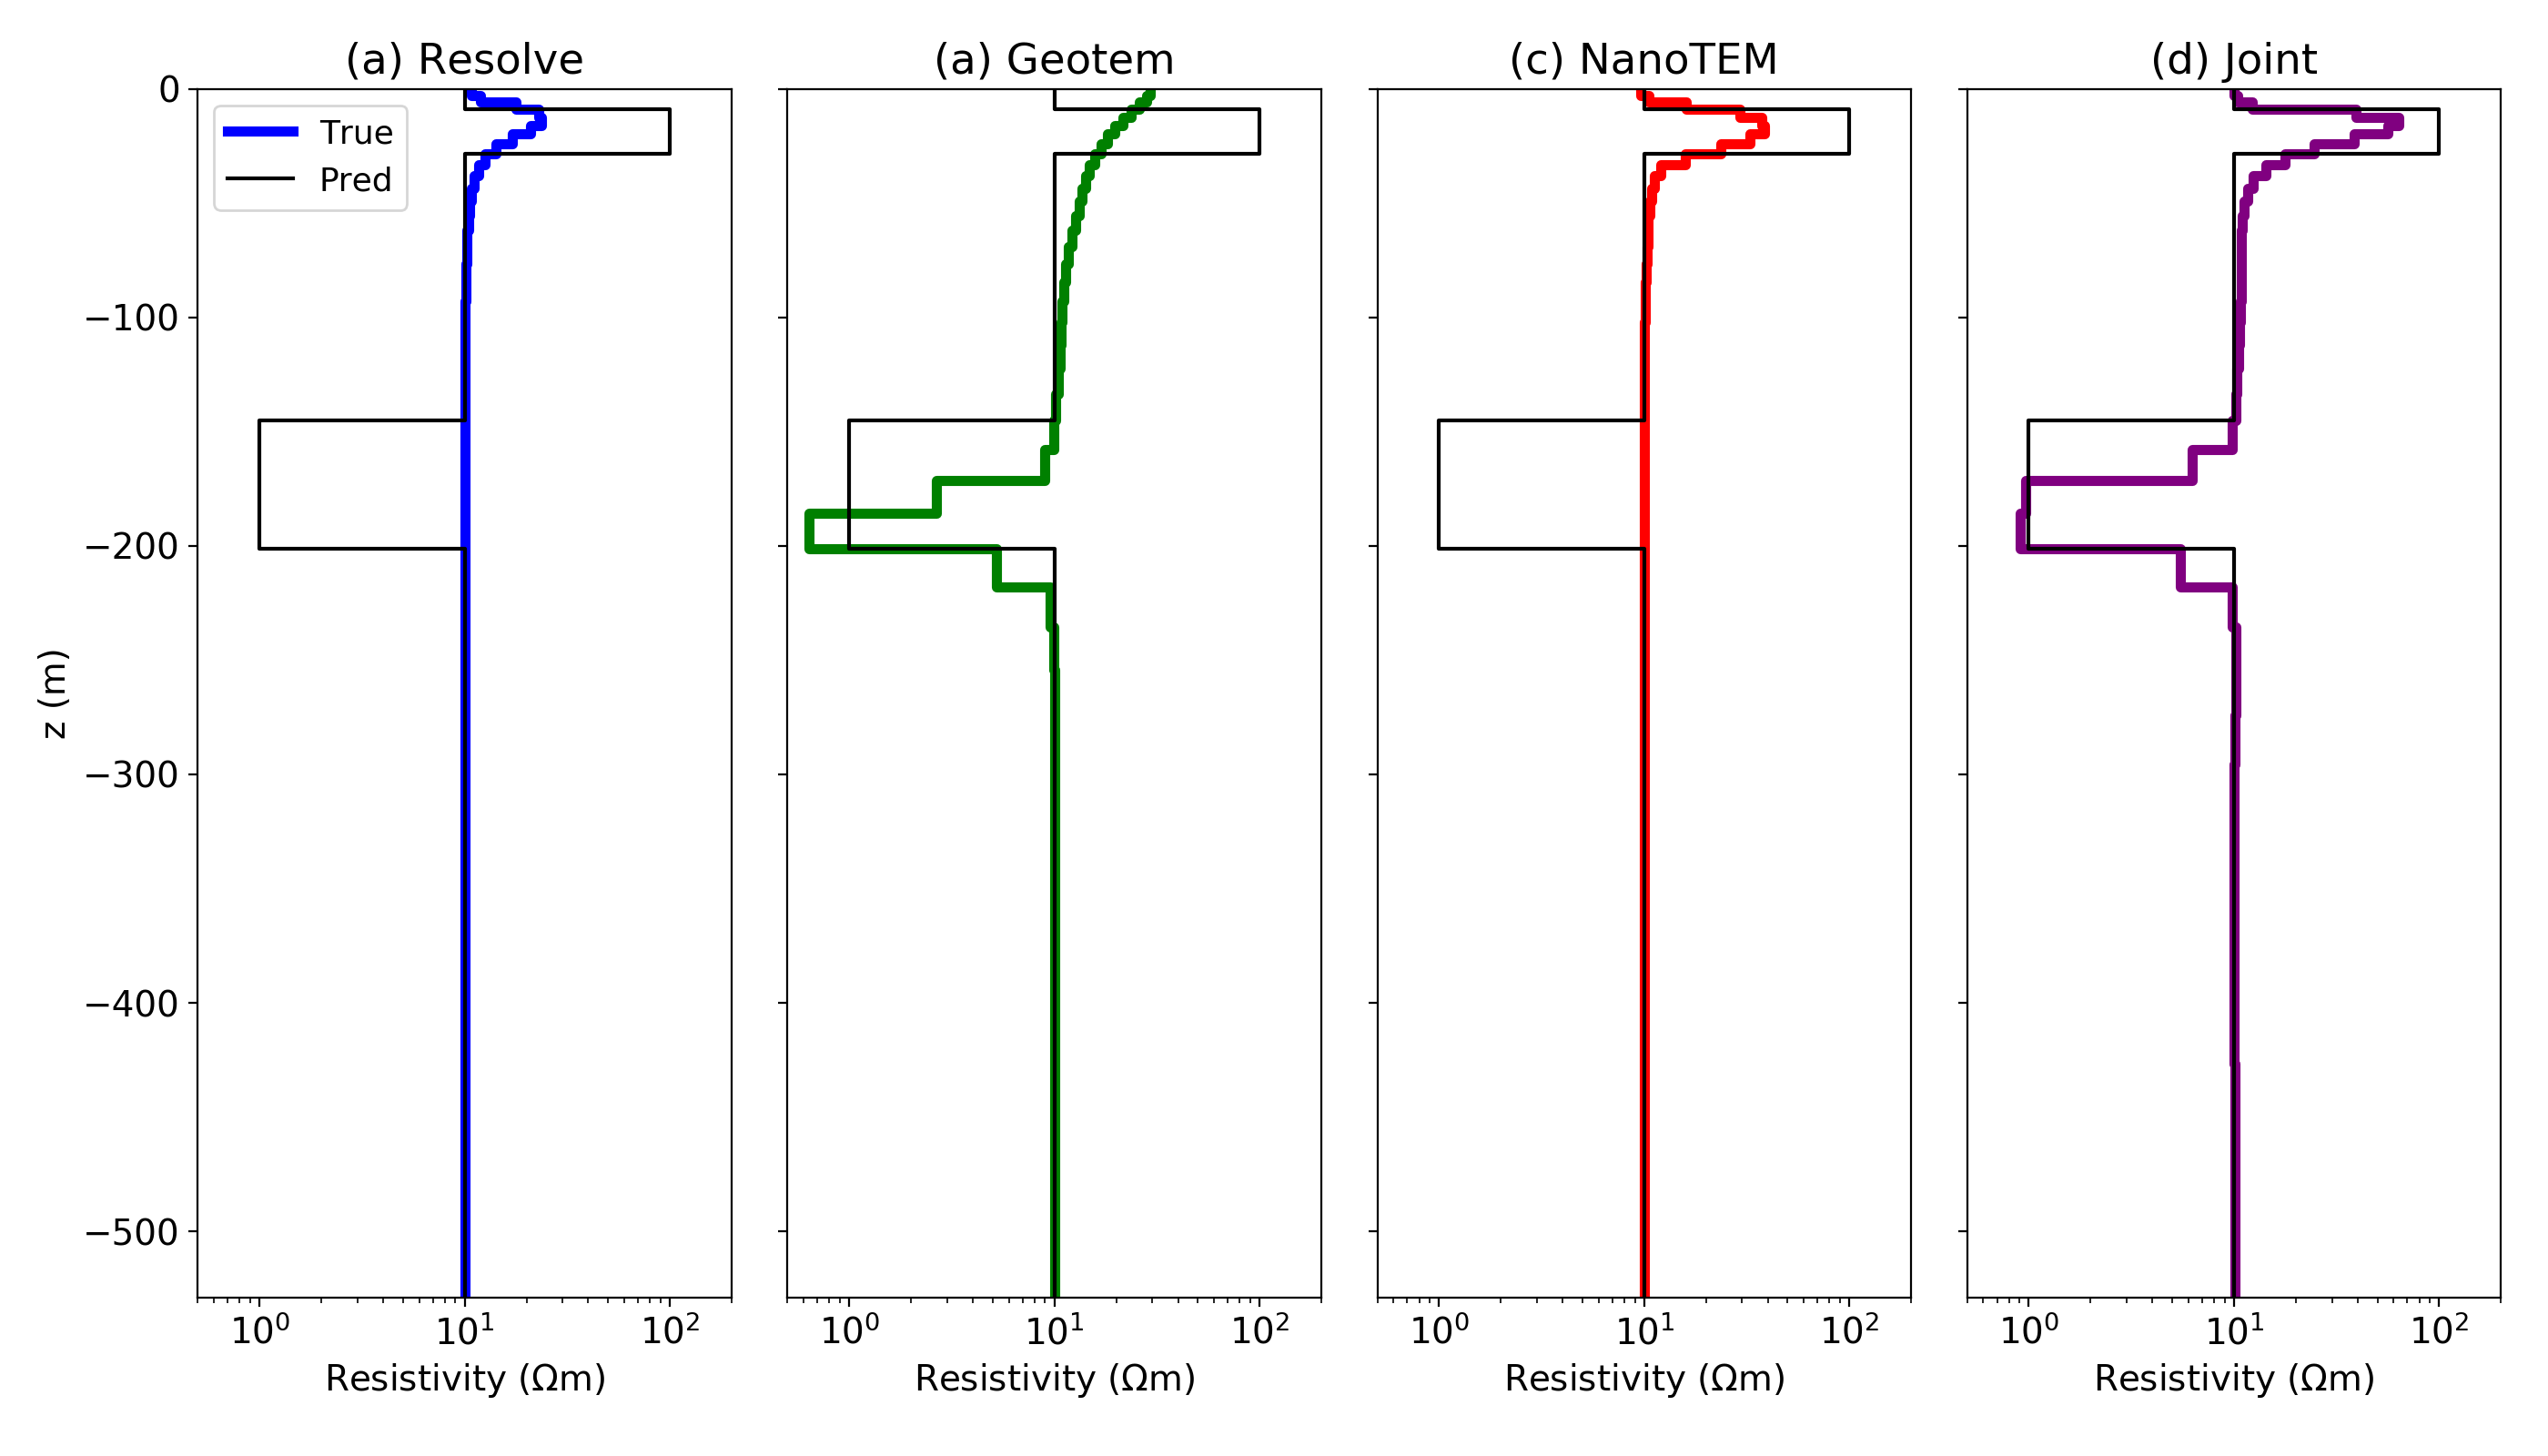
\includegraphics[width=0.8\columnwidth]{figures/blocky-inversion.png}
    \end{center}
\caption{
    Models recovered by performing an inversion employing a blocky norm with:
    (a) the Resolve data (airborne FDEM), (b) the Geotem data (airborne TDEM), (c) the NanoTEM (ground TDEM) data and (d) jointly inverting all 3 data sets.
}
\label{fig:blocky-inversion}
\end{figure}

